\documentclass{beamer}
\mode<presentation>
\usetheme{Malmoe}
%gets rid of bottom navigation bars
\setbeamertemplate{footline}[page number]{}

%gets rid of navigation symbols
\setbeamertemplate{navigation symbols}{}

\usepackage{comment}

\usepackage{listings}
\usepackage{color}
\definecolor{mauve}{rgb}{0.58,0,0.82}

\lstset{frame=tb,
  language=Python,
  showstringspaces=false,
  columns=flexible,
  basicstyle={\small\ttfamily},
  numbers=none,
  keywordstyle=\color{blue},
  stringstyle=\color{mauve},
  breaklines=true,
  breakatwhitespace=true,
  tabsize=4
}

\title{BrainBuilder: Pseudocolumn}
\author{Luis Riquelme, Mike Gevaert}
\institute{Human Brain Project}
\date{\today}

\begin{document}

\begin{frame}
  \titlepage
\end{frame}

\section{Introduction}
\subsection{Teaser}
\begin{frame}
  \frametitle{Replication the column using BrainBuilder}

  Which one is which?
  \begin{figure}[h]
    \fbox{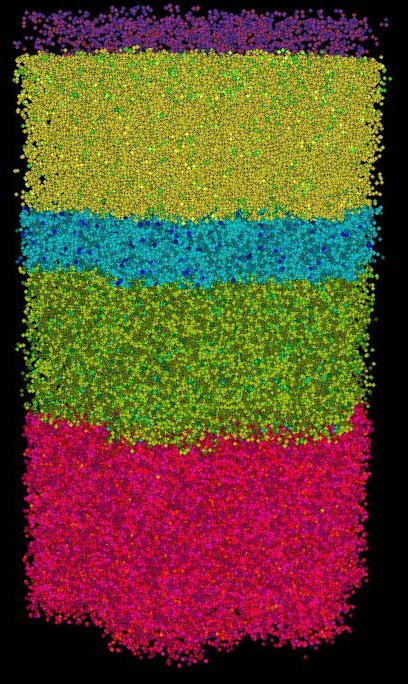
\includegraphics[height=0.5\textheight]{images/pseudo_column-v4.jpg}}
    \fbox{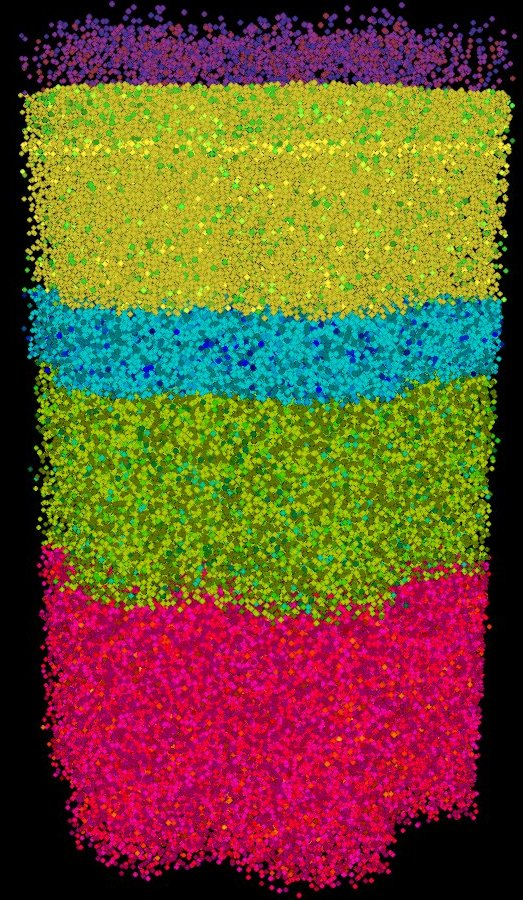
\includegraphics[height=0.5\textheight]{images/real_column_v5.jpg}}
  \end{figure}
\end{frame}

\begin{frame}
  \frametitle{Credit}
  Most of the work was done by Luis (but he's on vacation):
  \framebox{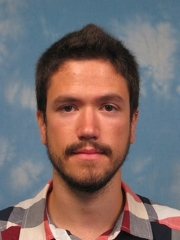
\includegraphics[height=0.5\textheight]{images/riquelme.jpg}}
\end{frame}

\subsection{Purpose}
\begin{frame}
  \frametitle{Purpose}
  \begin{itemize}
     \item See how well we can replicate the current column
     \item Have for check validation
     \item Have to do a 'vertical' column, since the later stages of the toolchain don't support arbitrary transformations
  \end{itemize}
\end{frame}

\section{Method}
\begin{frame}
  \frametitle{Generate Densities}
  Take the original column, and 'voxel-ize' it to produce a cell density map
  \begin{itemize}
     \item Based only on soma positions
     \item Do not look at ME-Type or sClass
  \end{itemize}
  \framebox{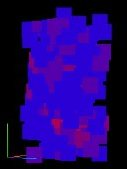
\includegraphics[height=0.5\textheight]{images/column_density.jpg}}
\end{frame}

\begin{frame}
  \frametitle{Generate Annotation Map}
  Take the original column, and 'voxel-ize' it to produce a cell annotation map
  \begin{itemize}
     \item Per voxel, gather all the cells, and the most popular layer label 'wins'
  \end{itemize}
  \framebox{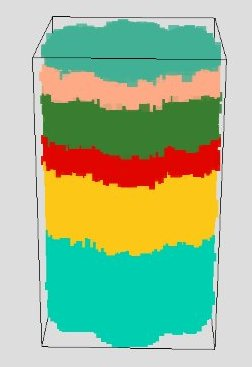
\includegraphics[height=0.5\textheight]{images/column_annotations.jpg}}
\end{frame}

\begin{frame}[fragile]
  \frametitle{Generate Annotation Hierarchy}
  Take the original column, and 'voxel-ize' it to produce a cell density map
  \begin{itemize}
     \item Can't use the stock Allen Institute one: they use 1, 2/3, 4, 5, 6a, 6b, as SSCx layers
     \item Want to use our XML recipe, so have the same dimensions
  \end{itemize}
  \lstinputlisting[lastline=10]{data/bbp_hierarchy_abbreviated.json}
\end{frame}

\begin{frame}
   \frametitle{Write Modules for BBP recipes}
  \begin{itemize}
     \item Create 'Spatial Distributions' using the recipe
     \begin{itemize}
        \item Need placement hints from NeuronDB.dat
        \item Need cell percentages from builderRecipeAllPathways.xml
     \end{itemize}
  \end{itemize}
\end{frame}

\section{Running}
\subsection{Build.Region}
\begin{frame}
  \frametitle{Select the Region}
  Select the whole column:

  \framebox{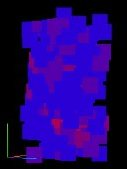
\includegraphics[height=0.5\textheight]{images/column_density.jpg}}
\end{frame}

\subsection{Build.Cells}
\begin{frame}
  \frametitle{Place the cell bodies}
  Colour doesn't mean anything, just needed contrast from different cells:

  \framebox{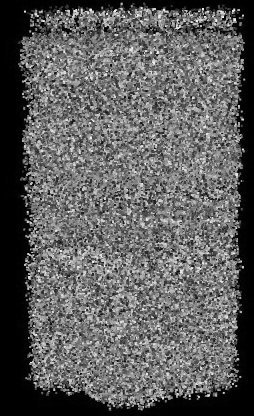
\includegraphics[height=0.5\textheight]{images/column_placed.jpg}}
\end{frame}

\begin{frame}
  \frametitle{Aside: Vector Fields}
  \begin{itemize}
     \item For each voxel, need the nearest voxel that isn't of the same annotation
     \item Green is 'Up', which is all we need for the SSCx at the moment
     \item Other colours are for more complicated modules, if necessary
  \end{itemize}
  \framebox{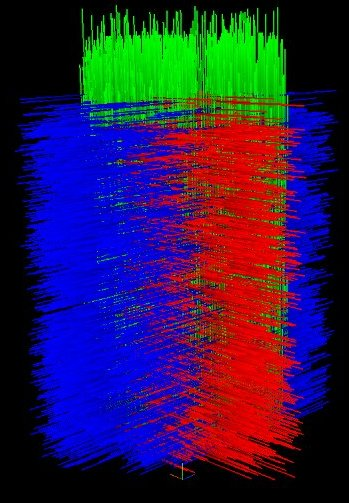
\includegraphics[height=0.5\textheight]{images/column_fields.jpg}}
\end{frame}

\subsection{Build.EI}
\begin{frame}
  \frametitle{Assign E-I-ness}
  Assign 'sclass' to cell bodies (Blue is Inhibitory):

  \framebox{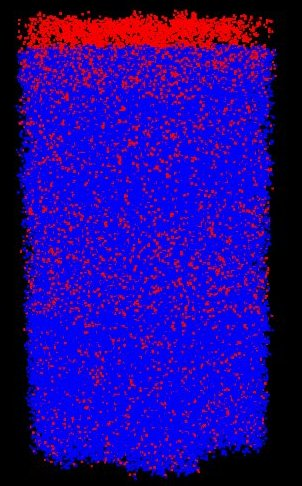
\includegraphics[height=0.5\textheight]{images/column_sclass.jpg}}
\end{frame}

\subsection{Build.Composition.ME}
\begin{frame}
  \frametitle{Assign ME-Types to cell bodies}
  E-Type (Sorry about the colours):

  \framebox{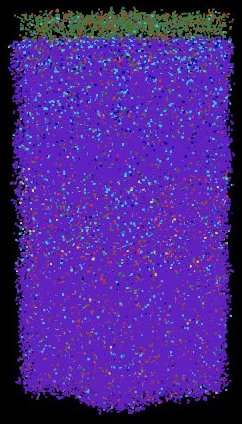
\includegraphics[height=0.5\textheight]{images/column_etype.jpg}}

  Note: ME-Types are assigned in the same module
\end{frame}

\subsection{Build.Composition.ME}
\begin{frame}
  \frametitle{Assign ME-Types to cell bodies}
  M-Type (Using same colour scheme as Platform column viewer):
  
  \framebox{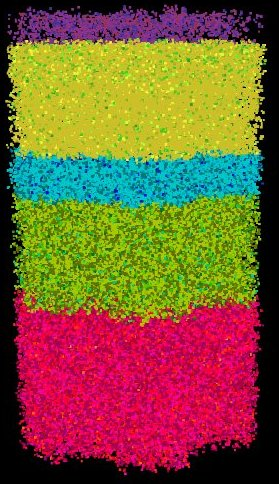
\includegraphics[height=0.5\textheight]{images/column_mtype.jpg}}
\end{frame}

\subsection{Build.Placement}
\begin{frame}
  \frametitle{Assign morphologies to cell bodies}
  Each morphology is assigned a different colour:

  \framebox{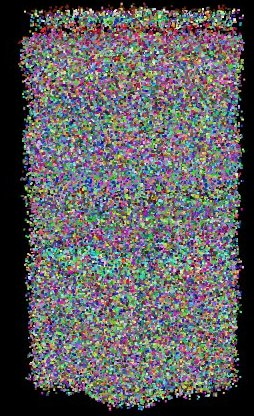
\includegraphics[height=0.5\textheight]{images/column_morph.jpg}}
\end{frame}

\section{Future}
\begin{frame}
  \frametitle{Future work}

  \begin{itemize}
     \item Can synthesize the 'whole' brain, including 3D orientations, need new format to describe this freedom
     \item The scale of this pseudo-column matches the old column, so rat morphologies work, however the Allen Institute map is mouse.  We can scale the voxel sizes appropritately
     \item Currently not worrying about, but that should be addressed:
     \begin{itemize}
        \item Colliding soma positions
        \item Morphologies protruding out of bounds
        \item Coarseness of Allen Institute annotations: causes weird artifacts.  Csaba has ways around this.
     \end{itemize}
  \end{itemize}
\end{frame}

\end{document}
